\documentclass[10pt,svgnames,usenames,table]{beamer} 

\NeedsTeXFormat{LaTeX2e}

\usetheme[compress]{Singapore} % theme

\usepackage[french]{babel}
\usepackage[T1]{fontenc}
\usepackage[utf8x]{inputenc}
\usepackage{lmodern}
\usepackage{amsmath,amsthm,amssymb}        % un packages mathématiques
\usepackage{pifont}
\newcommand{\cmark}{\ding{51}}%
\newcommand{\xmark}{\ding{55}}%
\usepackage{xcolor}         % pour définir plus de couleurs
\usepackage{graphicx}       % pour insérer des figures
\usepackage{lmodern}
\usepackage{url}
	\urlstyle{sf}
\usepackage{lastpage}
\usepackage{endnotes}

\usepackage{listings}
\usepackage{listingsutf8}

\usepackage{siunitx}
\usepackage{circuitikz}
\usepackage{chemfig}
\usepackage[version=3]{mhchem}

\usepackage[french]{varioref}
\usepackage{wrapfig}
\usepackage{pdfpages}
\usepackage{verbatim}
\usepackage{graphicx}

\usepackage{setspace}

%\usepackage[svgnames]{color}
%\definecolor{webdarkblue}{rgb}{0,0,0.4}
%\definecolor{webgreen}{rgb}{0,0.3,0}
%\definecolor{webblue}{rgb}{0,0,0.8}

\setbeamercolor{section in head/foot}{use=structure,bg=structure.fg!25!bg} % "Amélioration du jeu de couleur"
%\useoutertheme[subsection=true]{smoothbars} % Pour avoir un rappel de la subsection
\setbeamerfont{frametitle}{series=\bfseries}
\setbeamertemplate{frametitle}[default][center] % Titre centré et bien placé.


% "Fioriture de style" : qd <x-> dans les item, les autres en gris clair
\beamertemplatetransparentcovered


% Comportement des itemize
\setbeamertemplate{itemize item}[ball]
\setbeamertemplate{itemize subitem}[triangle]
\setbeamertemplate{itemize subsubitem}[circle]

%\renewcommand\sfdefault{cmss} % Polices

% Les block arrondis et ombrés dans la couleur que je veux
\setbeamertemplate{blocks}[rounded][shadow=true]
\definecolor{normalBlockColor}{RGB}{255,255,255}
\definecolor{normalTitleBlockColor}{RGB}{0,0,102}
\definecolor{normalBlockTextColor}{RGB}{0,0,0}
\definecolor{normalBlockTitleTextColor}{RGB}{255,255,255}
\definecolor{exampleBlockColor}{RGB}{202,251,197}
\definecolor{exampleTitleBlockColor}{RGB}{166,241,158}
\definecolor{exampleBlockTextColor}{RGB}{0,0,0}
\definecolor{exampleBlockTitleTextColor}{RGB}{0,120,0}
\definecolor{alertBlockColor}{RGB}{248,218,218}
\definecolor{alertTitleBlockColor}{RGB}{244,108,108}
\definecolor{alertBlockTextColor}{RGB}{0,0,0}
\definecolor{alertBlockTitleTextColor}{RGB}{120,0,0}
\setbeamercolor*{block title}{fg=normalBlockTitleTextColor,bg=normalTitleBlockColor}
\setbeamercolor*{block body}{fg=normalBlockTextColor,bg=normalBlockColor}
\setbeamercolor*{block title alerted}{fg=alertBlockTitleTextColor,bg=alertTitleBlockColor}
\setbeamercolor*{block body alerted}{fg=alertBlockTextColor,bg=alertBlockColor}
\setbeamercolor*{block title example}{fg=exampleBlockTitleTextColor,bg=exampleTitleBlockColor}
\setbeamercolor*{block body example}{fg=exampleBlockTextColor,bg=exampleBlockColor}
\setbeamerfont{block title}{size={}}



%------------ fin style beamer -------------------

% Faire apparaître un sommaire avant chaque section
% \AtBeginSection[]{
%   \begin{frame}
%   \frametitle{Plan}
%   \medskip
%   %%% affiche en début de chaque section, les noms de sections et
%   %%% noms de sous-sections de la section en cours.
%   \small \tableofcontents[currentsection, hideothersubsections]
%   \end{frame}
% }


% Pour personnaliser la barre de navigation du dessous
\setbeamertemplate{navigation symbols}{
	%\insertslidenavigationsymbol
	%\insertframenavigationsymbol
	%\insertsubsectionnavigationsymbol
	\quad\textbf{\insertframenumber/\inserttotalframenumber} % Numéro de page
	%\insertsectionnavigationsymbol
	%\insertdocnavigationsymbol
	%\insertbackfindforwardnavigationsymbol
}
% Supprimer les icones de navigation (pour les transparents)
%\setbeamertemplate{navigation symbols}{}

% Mettre les icones de navigation en mode vertical (pour projection)
% \setbeamertemplate{navigation symbols}[vertical]

\newenvironment{itemize2}%
	{ \begin{list}%
		{$\bullet$}%
		{\setlength{\labelwidth}{30pt}%
		 \setlength{\leftmargin}{35pt}%
		 \setlength{\itemsep}{\parsep}}}%
	{ \end{list} }

\def\siecle#1{\textsc{\romannumeral #1}\textsuperscript{e}~siècle} % => le \siecle{19}

\definecolor{codeBlue}{rgb}{0,0,1}
\definecolor{webred}{rgb}{0.5,0,0}
\definecolor{codeGreen}{rgb}{0,0.5,0}
\definecolor{codeGrey}{rgb}{0.6,0.6,0.6}
\definecolor{webdarkblue}{rgb}{0,0,0.4}
\definecolor{webgreen}{rgb}{0,0.3,0}
\definecolor{webblue}{rgb}{0,0,0.8}
\definecolor{orange}{rgb}{0.7,0.1,0.1}
\lstset{
      language=TeX,
      flexiblecolumns=true,
      numbers=left,
      stepnumber=1,
      numberstyle=\ttfamily\tiny,
      keywordstyle=\ttfamily\textcolor{blue},
      stringstyle=\ttfamily\textcolor{red},
      commentstyle=\ttfamily\textcolor{codeGreen},
      breaklines=true,
      extendedchars=true,
      basicstyle=\ttfamily\scriptsize,
      showstringspaces=false,
      morekeywords={usepackage,documentclass,begin,textbf,textit,texttt,ref,includegraphics,caption,label,setlength,mathbb,notag,frac,num,si,ang,SI,textwidth,percent,meter,ohm,joule,second,more,section,subsection,tableofcontents,setstretch,TeX,LaTeX,huge,sffamily,emph,chemfig,pageref,vpageref,date,maketitle,institute,author,and,textsc,title,includeonly,include,clearpage,newcommand,mathsf,renewcommand,DeclareMathOperator,mathrm,captionof,lstinputlisting,lstinline},
      frame=single,
      extendedchars=true,
      inputencoding=utf8x,
	    literate={á}{{\'a}}1 {ã}{{\~a}}1 {é}{{\'e}}1 {è}{{\`e}}1 {à}{{\`a }}1
    }
\lstset{inputencoding=utf8/latin1}

\newsavebox\mybox
\newenvironment{aquote}[1]
{\savebox\mybox{#1}\begin{quote}}
{{{\leavevmode\unskip\nobreak\hfil\penalty50\hskip2em
    \hbox{}\nobreak\hfil(\usebox\mybox)%
\parfillskip=0pt \finalhyphendemerits=0 \endgraf}}\end{quote}}

%\setbeamertemplate{headline}{}

\usepackage{pdflscape} %% portrait
\usepackage[french]{varioref} % \vpageref
\usepackage{pgfplots}
\usepackage{framed}
\usepackage{mdframed}
\usepackage{epstopdf}
\usepackage{xspace}
\usepackage{caption}
\usepackage{subcaption}
\usepackage{menukeys}
\usepackage{comment}
\captionsetup[figure]{labelformat=empty}

\usepackage[colorinlistoftodos]{todonotes}%disable=true

\newcommand{\badet}{et}
\newcommand{\goodet}{\mathbin{\mathrm{et}}}
\DeclareMathOperator{\sumN}{\sum_{i=1}^n}
\DeclareMathOperator{\var}{\mathrm{Var}}

\lstdefinestyle{nonumbers}
{numbers=none}

% Pour rendre les toc plus compactes (pour éviter que ça déborde)
\makeatletter
\patchcmd{\beamer@sectionintoc}{\vskip1.5em}{\vskip0.5em}{}{}
\makeatother
\setbeamerfont{subsection in toc}{size=\scriptsize}

\setbeamertemplate{frametitle continuation}{}

\graphicspath{{Images/}}
\definecolor{gris}{RGB}{228,228,228}
\definecolor{bleu}{RGB}{34,148,255}
\definecolor{darkgray}{rgb}{0.3,0.3,0.3}
\usefonttheme[onlymath]{serif} % to see the difference when I do mathsf

\logo{
\includegraphics[height=5mm]{Images/logo_12-13-mini}}
\institute{Louvain-li-Nux}
\title{\textbf{Formation GIMP}\\
Introduction au montage photo avec GIMP}
\author{Adrien~\textsc{Couplet} \and Sébastien~\textsc{de Longueville} \and Laurent~\textsc{Ziegler}}

\date{5 avril 2018}


\begin{document}

\begin{frame}
	\maketitle
\end{frame}

\begin{frame}
  \begin{center}\Large
  Suivez cette présentation sur votre ordinateur :-)
  
  \vspace{1cm}
  \fbox{\url{https://louvainlinux.org/activites/atelier-gimp}}
  \end{center}
\end{frame}

\section{Introduction}
\begin{frame}[allowframebreaks]{Qu'est-ce que GIMP ?}
    \begin{itemize}
        \item GIMP = GNU Image Manipulation Program
        \item Logiciel de traitement d'images bitmap.
        \item Alternative gratuite et libre à Adobe Photoshop
    \end{itemize}
    \begin{figure}
        \centering
        
\includegraphics[width=0.5\textwidth]{Images/gimp-logo}
        \caption{Wilber, la mascotte officielle de GIMP} 
    \end{figure}
    \framebreak
    Liste non exhaustive des fonctionnalités de GIMP
    \begin{itemize}
        \item Gestion des calques;
        \item Plusieurs outils de dessin;
        \item Plusieurs outils de sélection;
        \item Outils de transformation;
        \item Une sélection de filtres;
        \item Gestion de nombreux formats (JPEG, GIF, PNG, PSD, TIFF);
        \item ...
    \end{itemize}
\end{frame}

\begin{frame}{Installation}
    \begin{center}
    GIMP est disponible pour Windows, Linux et macOS
    \vspace{1cm}\Large
    \fbox{\url{https://www.gimp.org/downloads/}}
    \end{center}
\end{frame}

\section{Présentation de l'interface et des outils}
\begin{frame}[allowframebreaks]{L'interface}
    \begin{figure}
        \centering
        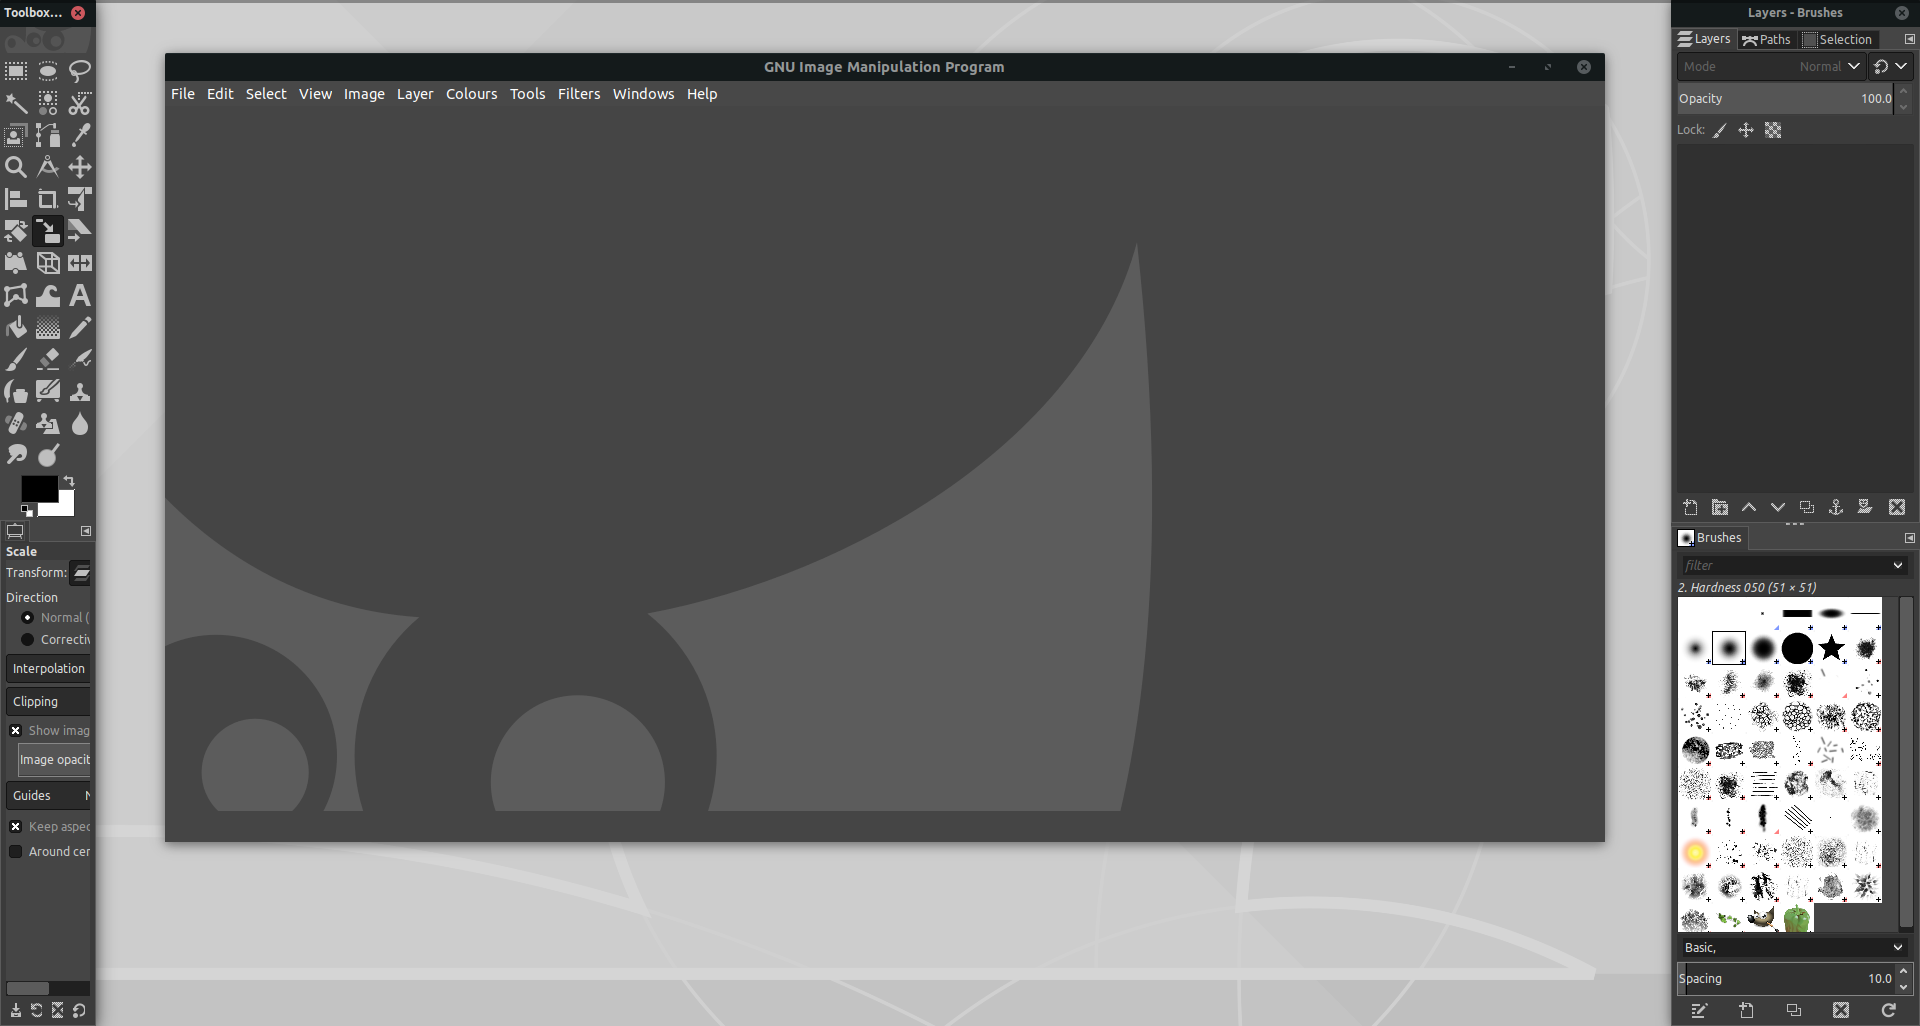
\includegraphics[width=0.9\textwidth]{Images/gimp_multiple_windows}
        \caption{L'interface multi-fenêtres}
    \end{figure} 
    \framebreak
    \begin{center}
        Fenêtres > Mode fenêtre unique
        \begin{figure}
            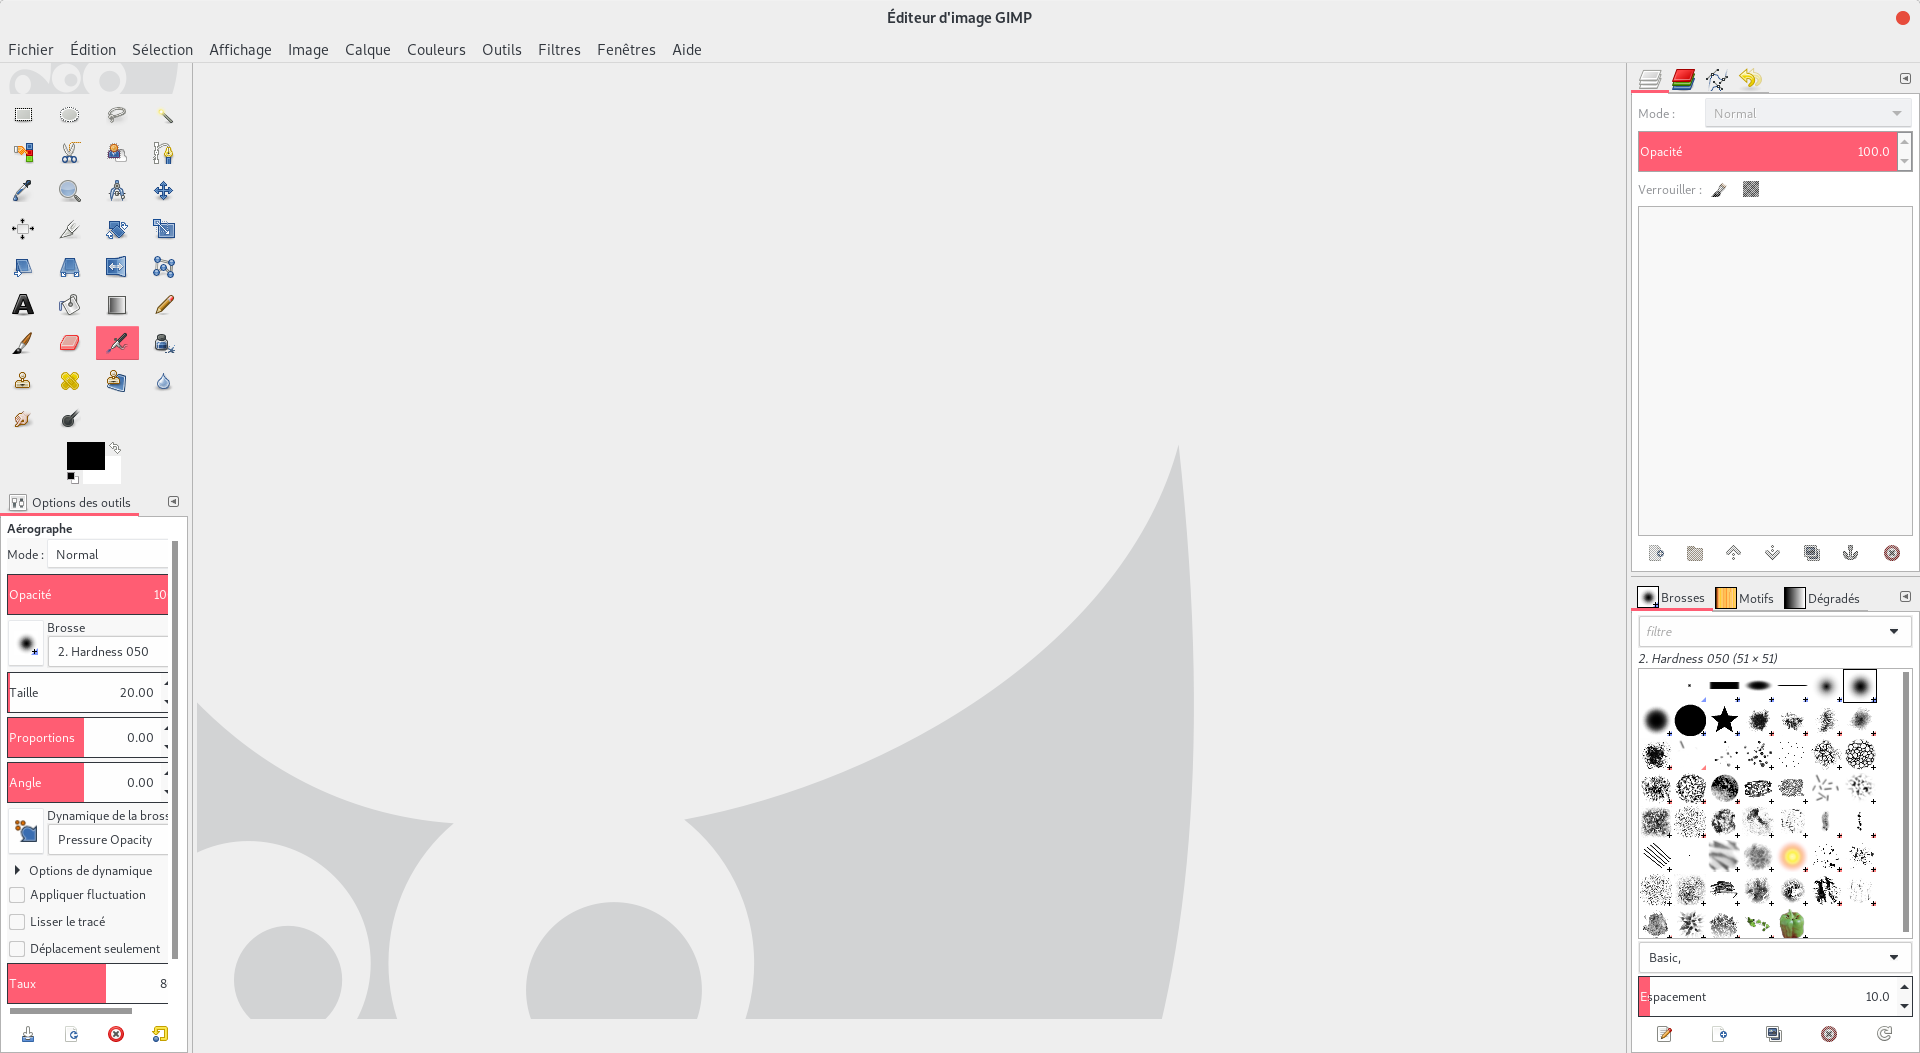
\includegraphics[width=0.9\textwidth]{Images/gimp_single_window}
            \caption{L'interface fenêtre unique}
        \end{figure}
    \end{center}
\end{frame}

\begin{frame}{Créer/importer une image}
	\begin{itemize}
		\item Pour \textbf{créer} une image: Fichier > Nouvelle image ou \keys{\ctrl + N}
			\begin{itemize}
				\item Sélectionnez un modèle (A3, A4, A5...) ou spécifier manuellement les dimensions (en pixels, mm, cm...).
			\end{itemize}
		\item Pour \textbf{importer} une image: Fichier  > Ouvrir ou \keys{\ctrl + O}.
			\begin{itemize}
				\item GIMP supporte de nombreux formats: PNG, JPEG, GIF...
			\end{itemize}
		\item Pour \textbf{créer} depuis le presse-papiers (copier/coller): Créer > Depuis le presse-papiers ou \keys{\shift + \ctrl + V}
	\end{itemize}
	\begin{center}
		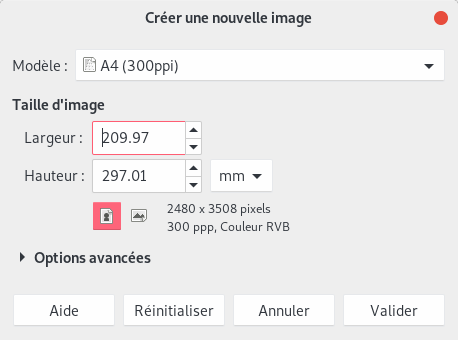
\includegraphics[width=0.5\textwidth]{Images/new_image.png}
	\end{center}
\end{frame}

\begin{frame}{Une image c'est quoi ?}
	\begin{center} 
		\textbf{Image matricielle} $\leftrightarrow$ Image vectorielle 
		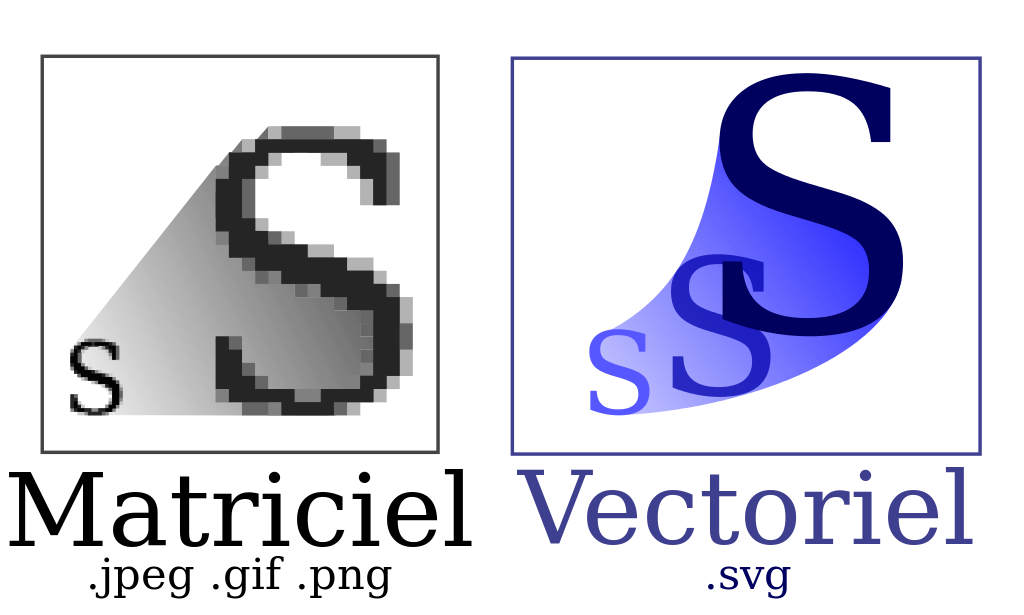
\includegraphics[width=0.6\textwidth]{Images/mat_vs_vec}
	\end{center}
	Pourquoi on utilise pas toujours des images vectorielles ? 
	\begin{itemize}
		\item les images vectorielles ne peuvent afficher que des images construites à l'aide de formes. Les images matricielles ont l'avantage d'être définies au pixel près.
	\end{itemize}
\end{frame}

\begin{frame}{Les formats}
	Stocker chaque pixel demande beaucoup de mémoire. Solution ? Compresser les images:
	\begin{itemize}
		\item compression sans pertes (PNG, GIF);
		\item compression avec pertes (JPEG).
	\end{itemize}
	Les trois principaux formats d'images sont
	\begin{itemize}
		\item \textbf{JPEG}: léger (mais avec pertes), idéal pour les photos;
		\item \textbf{PNG}: plus lourd que JPEG (mais sans pertes), très bon support de la transparence;
		\item \textbf{GIF}: support des animations, limité à 256 couleurs.
	\end{itemize}
	Un projet GIMP sera sauvegardé au format \textbf{XCF}, un format d'image libre qui contiendra les différents calques et paramètres de votre création.
	
	L'équivalent d'Adobe Photoshop est le format \textbf{PSD}.
\end{frame}

\begin{frame}{Enregistrement et exportation}
	\begin{itemize}
		\item Pour \textbf{enregistrer} au format \textbf{XCF}: Fichier > Enregistrer ou \keys{\ctrl + S}.
		\item Pour \textbf{exporter} votre image dans un autre format: Fichier > Exporter ou \keys{\shift + \ctrl + E}.
	\end{itemize}
	\begin{center}
		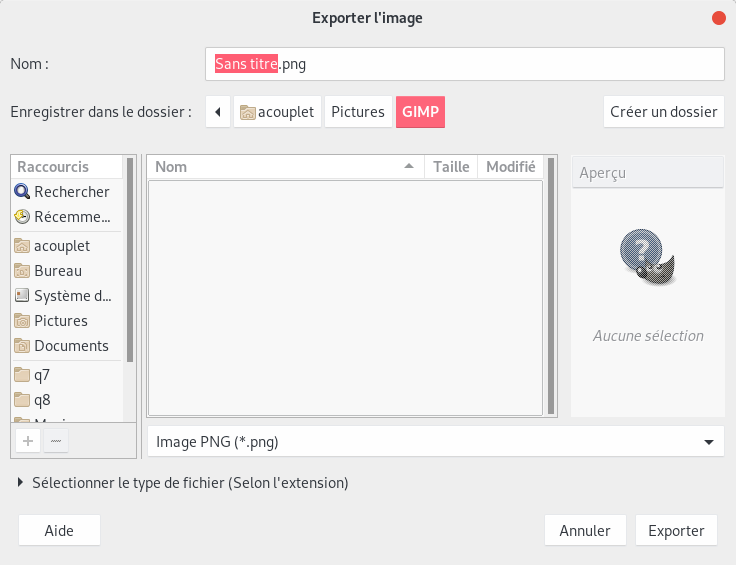
\includegraphics[width=0.5\textwidth]{Images/export}
	\end{center}
\end{frame}

\begin{frame}{Les couleurs}
	Il est possible de gérer 2 couleurs: les couleurs de premier et d'arrière-plan:
	\begin{center}
		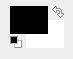
\includegraphics[width=0.08\textwidth]{Images/color_primary}
	\end{center}
	Il suffit de cliquer sur une de ces couleurs pour la modifier:
	\begin{center}
		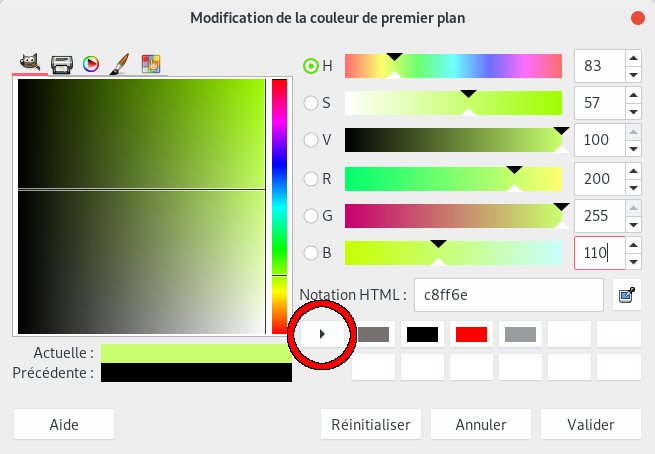
\includegraphics[width=0.5\textwidth]{Images/color_selector}
	\end{center}
	Il est possible de sélectionner une couleur ou de rentrer ses valeurs RGB. Une fois votre couleur choisie, vous pouvez l'ajouter à votre palette.
\end{frame}

\begin{frame}[allowframebreaks]{Les outils de coloration}
	La \textbf{pipette} permet de récupérer la couleur d'un pixel d'une image en cliquant sur le pixel en question.
	\begin{center}
		
\includegraphics[width=0.05\textwidth]{Images/color_tool_0}
		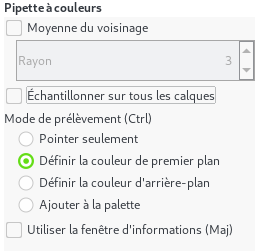
\includegraphics[width=0.3\textwidth]{Images/color_tool_0_settings}
	\end{center}
	L'outil permet de définir la couleur de premier plan, la couleur d'arrière-plan ou simplement d'ajouter la couleur à la palette.
	
	\framebreak
	Le \textbf{pot de peinture} permet de remplir une zone.
	\begin{center}
		
\includegraphics[width=0.05\textwidth]{Images/color_tool_1}
		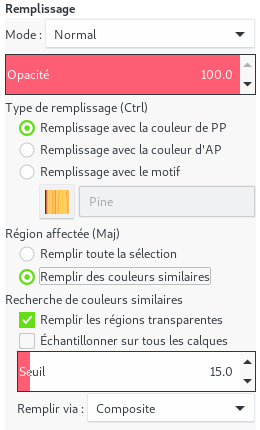
\includegraphics[width=0.25\textwidth]{Images/color_tool_1_settings}
	\end{center}
	Le seuil permet d'ajuster la zone à remplir: 
	\begin{center}
		
\includegraphics[width=0.3\textwidth]{Images/color_tool_1_test0}
		
\includegraphics[width=0.3\textwidth]{Images/color_tool_1_test1}
		
\includegraphics[width=0.3\textwidth]{Images/color_tool_1_test2}
	\end{center}
	\begin{scriptsize}
	Exemple: image originale, remplissage noir avec seuil à 30, remplissage noir avec seuil à 60.
	\end{scriptsize}
	
	\framebreak
	L'outil de gradient permet de créer des dégradés entre la couleur de premier plan et celle d'arrière-plan.
	\begin{center}
		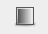
\includegraphics[width=0.05\textwidth]{Images/color_tool_2}
		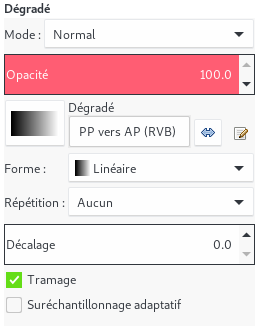
\includegraphics[width=0.3\textwidth]{Images/color_tool_2_settings}
	\end{center}
	Il existe de nombreux modes et de nombreuses formes, n'hésitez pas à les essayer pour les découvrir. 
	
\end{frame}

\begin{frame}[allowframebreaks]{Les outils}
	
	\begin{figure}
        	\centering
        	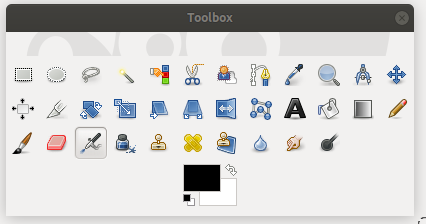
\includegraphics[width=0.4\textwidth]{Images/gimp_toolbox}
        	\caption{La boite à outils de GIMP} 
    	\end{figure}
	
	\textbf{Accès}
	
	\begin{itemize}
		\item Fenêtres > Boite à outils
		\item Outils > Boite à outils
	\end{itemize}
	
	\vspace{0.2cm}
	\textbf{Raccourci} \keys{\ctrl + B}
	
	\framebreak
	\textbf{Paramètres} \textit{double} cliquer sur l'icone l'outil concerné
	\begin{figure}
        	\centering
        	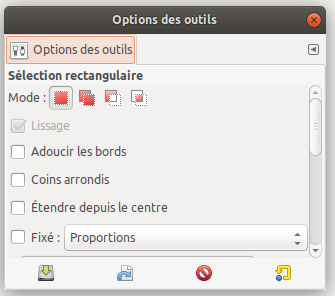
\includegraphics[width=0.4\textwidth]{Images/option_outil}
        	\caption{Exemple : paramètres de l'outil de sélection} 
    	\end{figure}

\end{frame}	

\begin{frame}[allowframebreaks]{Les outils de sélection}
\todo[inline]{icones outils \& Image résultat \& Interfaces}
\begin{enumerate}
	\item Rectangulaire \keys{R}
	
	Options : 
		
	\begin{itemize}
		\item Position
		\item Proportions fixées
		\item Hauteur fixée
		\item Largeur fixée
	\end{itemize}
	
	\framebreak
	
	\item Elliptique \keys{E}
	
	Options : 
		
	\begin{itemize}
		\item Position
		\item Proportions fixées
		\item Hauteur fixée
		\item Largeur fixée
	\end{itemize}
	
	\framebreak 
	
	\item Ciseaux intelligents \keys{I}
	
	\textbf{Attention} Une fois le contour terminer, cliquer au \textbf{centre} de celui-ci pour le valider
	\item A main levée \keys{F}
	\begin{itemize}
		\item \textbf{Trait continu} Maintenier le clic gauche 
		\item \textbf{Point par point} Clic sur chaque point successif 
	\end{itemize} 
	\item Par couleur \keys{Maj + O}
\end{enumerate}
\end{frame}

\begin{frame}{Les outils de sélection}
\textbf{Paramètres de sélection}
\begin{figure}
        \centering
        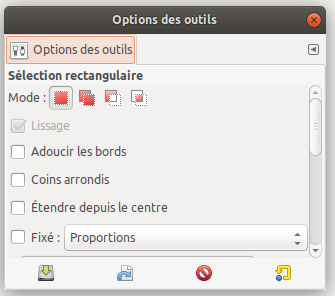
\includegraphics[width=0.4\textwidth]{Images/option_outil} 
\end{figure}

\begin{enumerate}
	\item \textbf{Remplacer} la sélection actuelle
	\item \textbf{Ajouter} à la sélection actuelle
	\item \textbf{Soustraire} à la sélection actuell
	\item \textbf{Intersection} avec la sélection actuelle	
\end{enumerate}
\end{frame}

\begin{frame}{Les outils de sélection}
\textbf{Paramètres de sélection}
\begin{overprint}
\begin{figure}
        \centering
        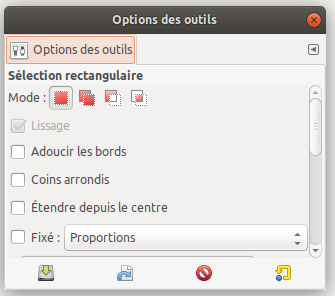
\includegraphics[width=0.4\textwidth, trim = 0 6.3cm 0 0, clip]{Images/option_outil} 
\end{figure}

\begin{enumerate}

	\only<1>{
	\item \textbf{Exemple}
	\begin{figure}
        	\centering
        	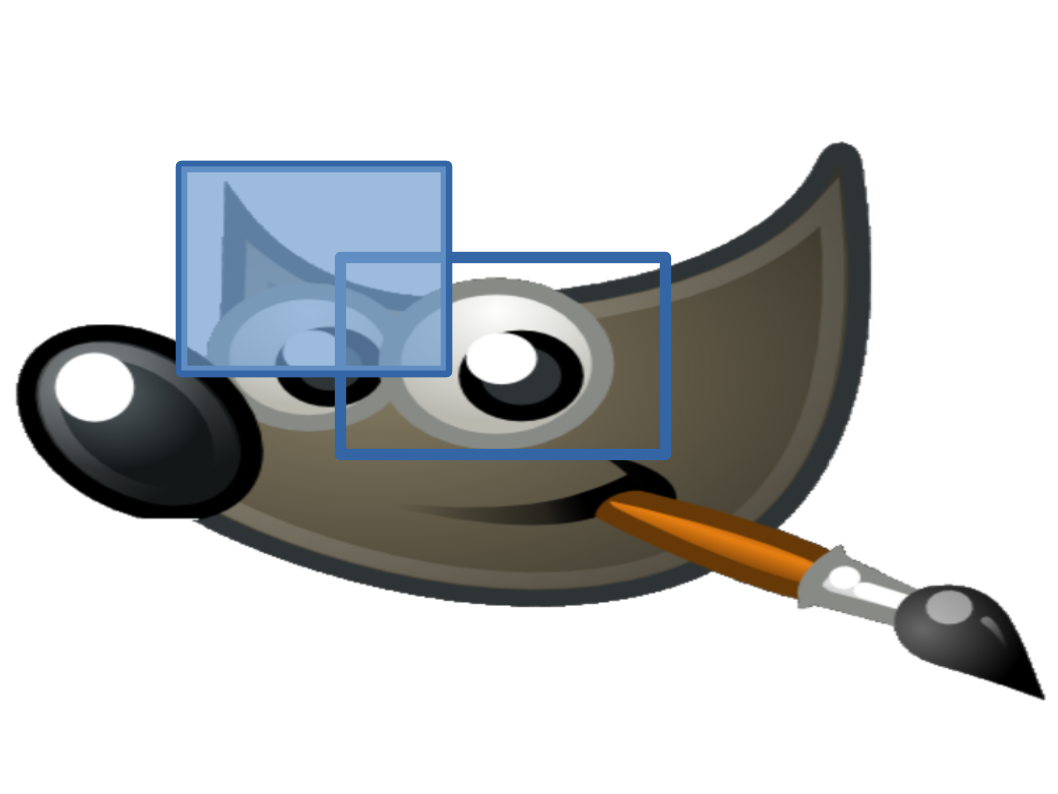
\includegraphics[width=0.4\textwidth]{Images/Selec1.png} 
	\end{figure}}
	
	\only<2>{
	\item[1] \textbf{Remplacer} la sélection actuelle
	\begin{figure}
        	\centering
        	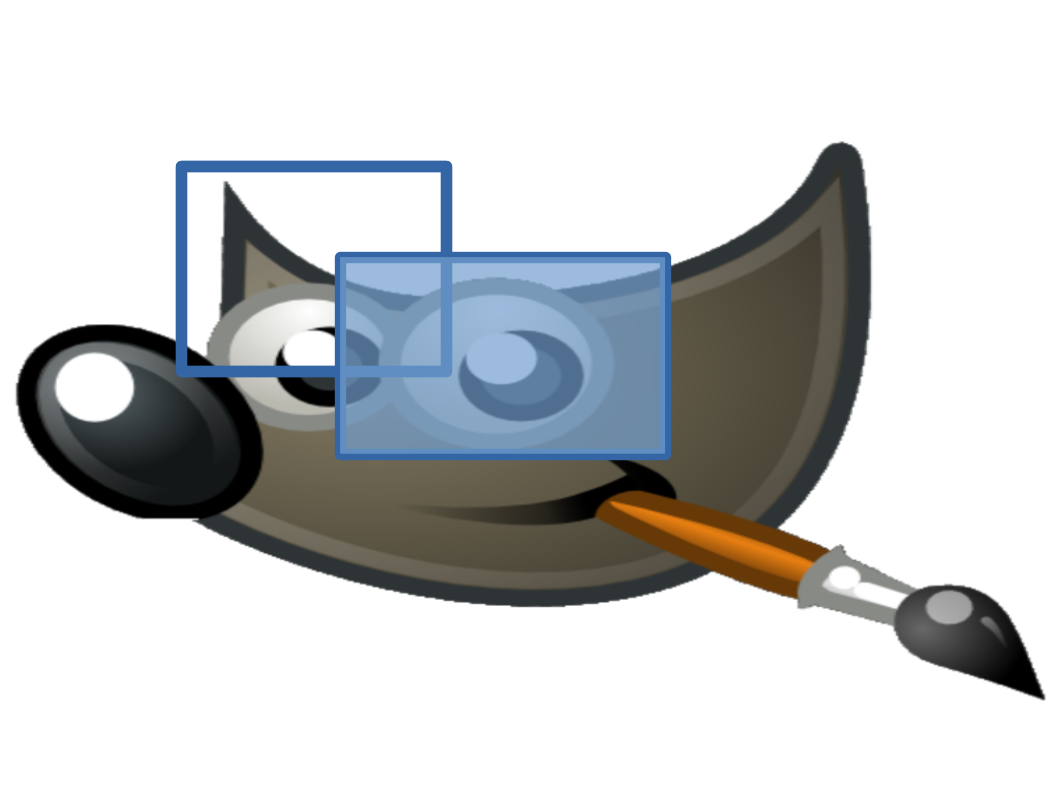
\includegraphics[width=0.4\textwidth]{Images/Selec5.png} 
	\end{figure}}
	
	\only<3>{	
	\item[2] \textbf{Ajouter} à la sélection actuelle
	\begin{figure}
        	\centering
        	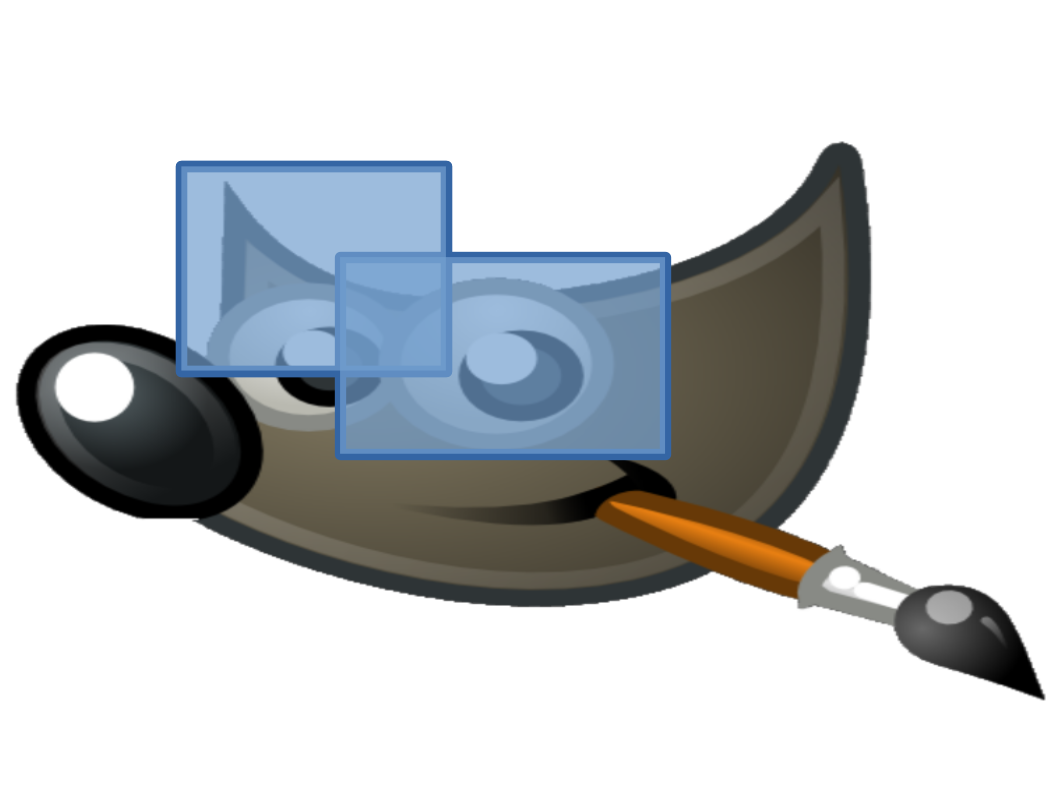
\includegraphics[width=0.4\textwidth]{Images/Selec2.png} 
	\end{figure}}
	
	\only<4>{
	\item[3] \textbf{Soustraire} à la sélection actuelle
	\begin{figure}
        	\centering
        	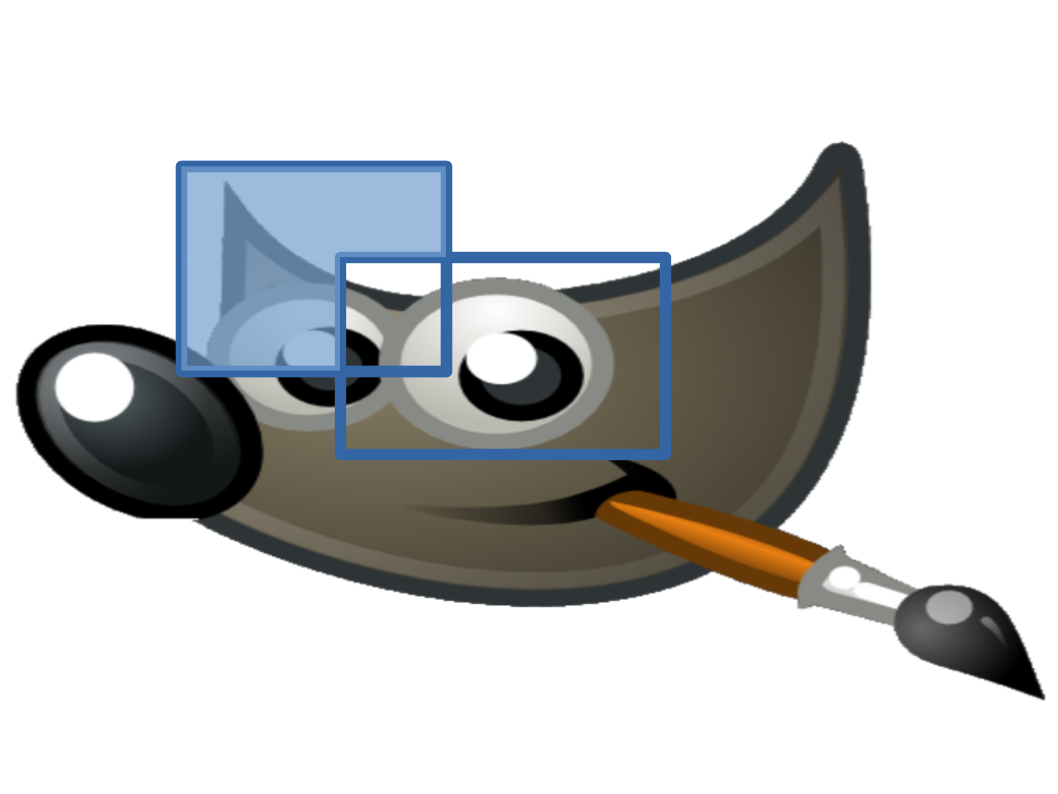
\includegraphics[width=0.4\textwidth]{Images/Selec3.png} 
	\end{figure}}
	
	\only<5>{
	\item[4] \textbf{Intersection} avec la sélection actuelle
	\begin{figure}
        	\centering
        	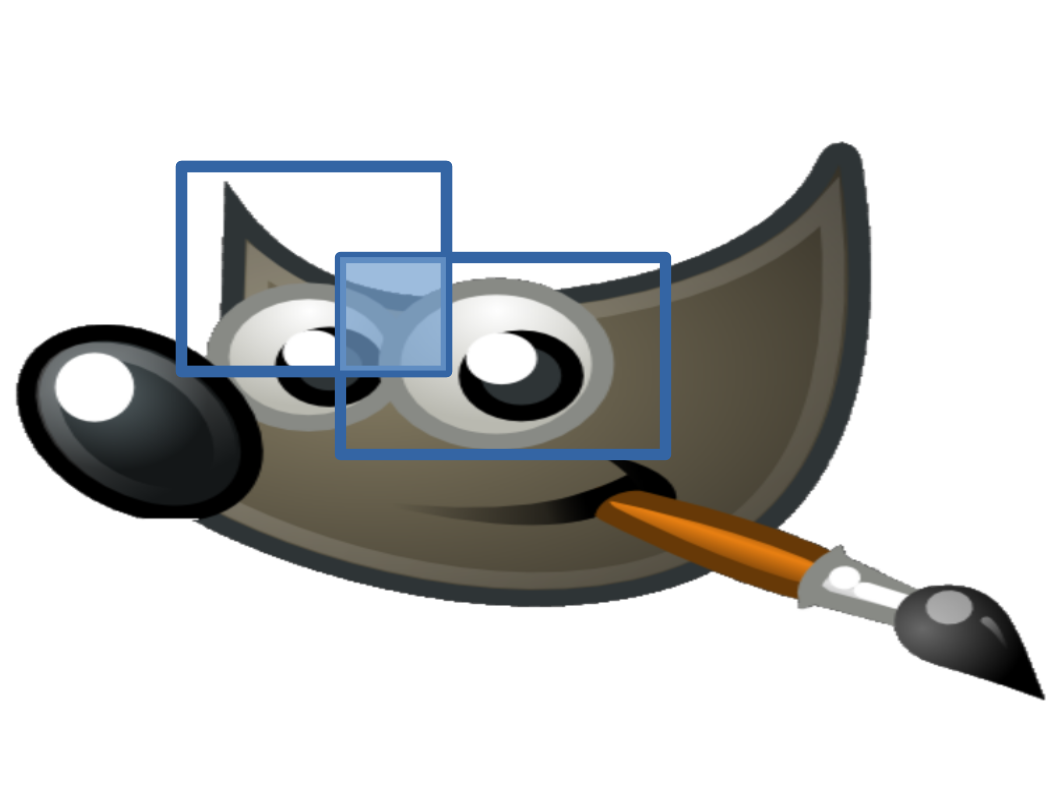
\includegraphics[width=0.4\textwidth]{Images/Selec4.png} 
	\end{figure}}
	
\end{enumerate}
\end{overprint}
\end{frame}

\begin{frame}[allowframebreaks]{Les outils de transformation}
\begin{enumerate}
	\item Rotation \keys{Maj + R}
	
	\begin{minipage}{0.45\textwidth}
	\begin{figure}
        	\centering
        	
\includegraphics[width=\textwidth]{Images/gimp-logo.png} 
	\end{figure}
	\end{minipage}\hfill
	\begin{minipage}{0.45\textwidth}
	\begin{figure}
        	\centering
        	
\includegraphics[width=0.8\textwidth]{Images/Rotate.png} 
	\end{figure}
	\end{minipage}
	\framebreak
	
	\item Agrandissement/Réduction \keys{Maj + T}
	
	\begin{minipage}{0.45\textwidth}
	\begin{figure}
        	\centering
        	
\includegraphics[width=\textwidth]{Images/gimp-logo.png} 
	\end{figure}
	\end{minipage}\hfill
	\begin{minipage}{0.45\textwidth}
	\begin{figure}
        	\centering
        	
\includegraphics[width=\textwidth]{Images/Flip.png} 
	\end{figure}
	\end{minipage}
	\framebreak
	
	\item Inversion \keys{Maj + F}
	
	\begin{minipage}{0.45\textwidth}
	\begin{figure}
        	\centering
        	
\includegraphics[width=\textwidth]{Images/gimp-logo.png} 
	\end{figure}
	\end{minipage}\hfill
	\begin{minipage}{0.45\textwidth}
	\begin{figure}
        	\centering
        	
\includegraphics[width=\textwidth]{Images/Flip.png} 
	\end{figure}
	\end{minipage}
	
	\begin{minipage}{0.45\textwidth}
	\begin{figure}
        	\centering
        	
\includegraphics[width=\textwidth]{Images/gimp-logo.png} 
	\end{figure}
	\end{minipage}\hfill
	\begin{minipage}{0.45\textwidth}
	\begin{figure}
        	\centering
        	
\includegraphics[width=\textwidth]{Images/Flip2.png} 
	\end{figure}
	\end{minipage}
	\framebreak
	
	\item Cisaillement \keys{Maj + S}
	
	\begin{minipage}{0.45\textwidth}
	\begin{figure}
        	\centering
        	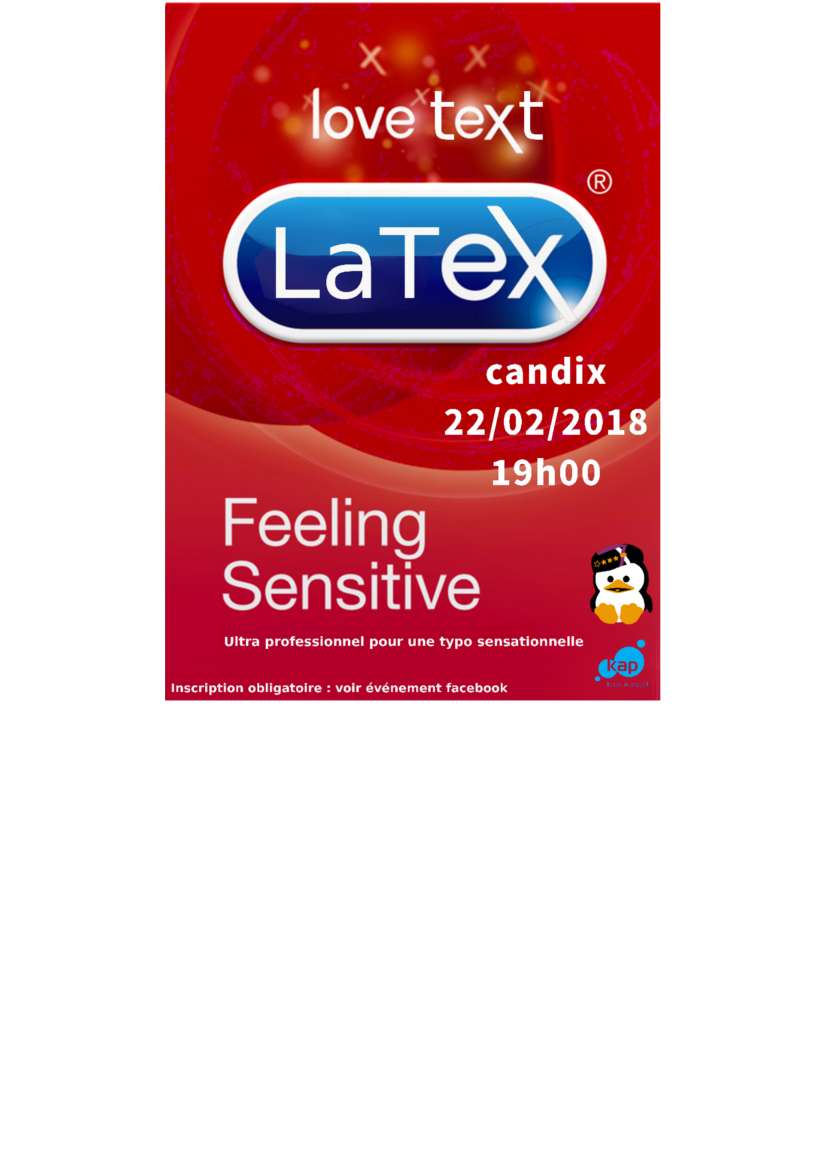
\includegraphics[width=\textwidth]{Images/NoShear.png} 
	\end{figure}
	\end{minipage}\hfill
	\begin{minipage}{0.45\textwidth}
	\begin{figure}
        	\centering
        	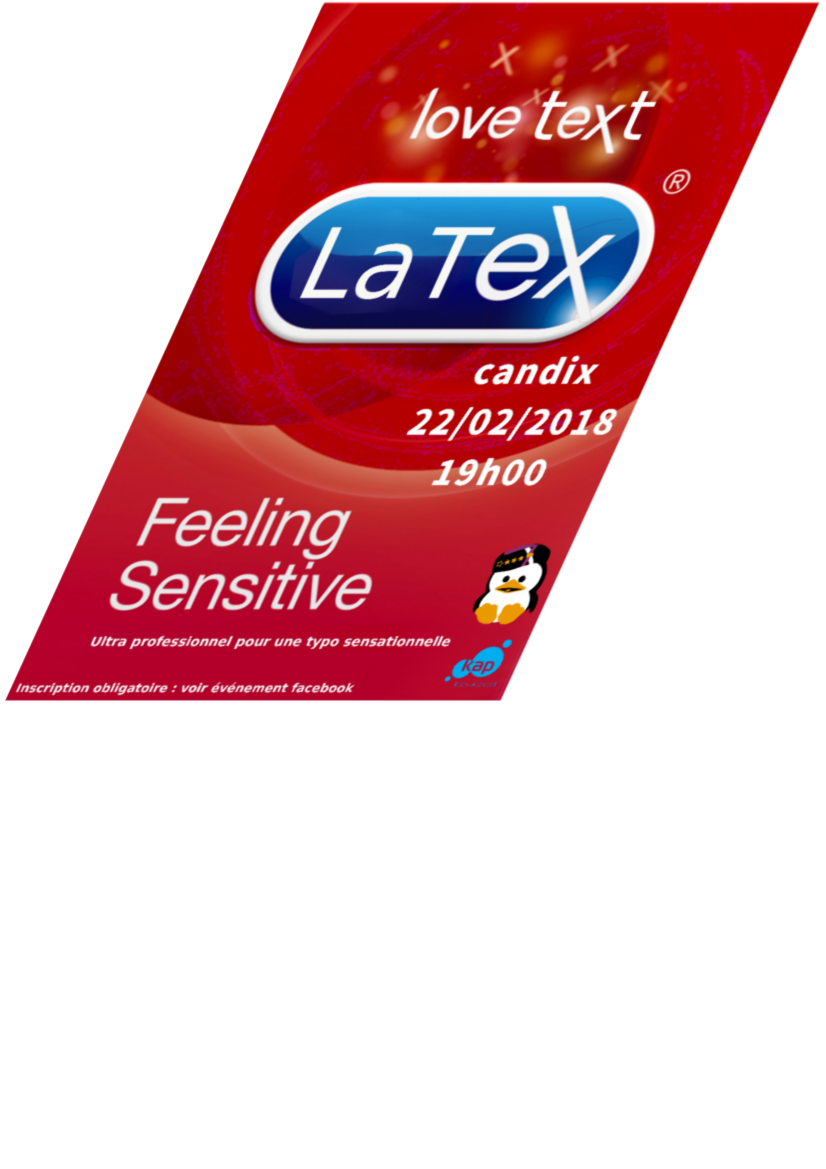
\includegraphics[width=\textwidth]{Images/Shear.png} 
	\end{figure}
	\end{minipage}
	\framebreak
	
	\item Mise en perspective \keys{Maj + R}
	
	\begin{minipage}{0.45\textwidth}
	\begin{figure}
        	\centering
        	
\includegraphics[width=0.5\textwidth]{Images/FullTex.png} 
	\end{figure}
	\end{minipage}\hfill
	\begin{minipage}{0.45\textwidth}
	\begin{figure}
        	\centering
        	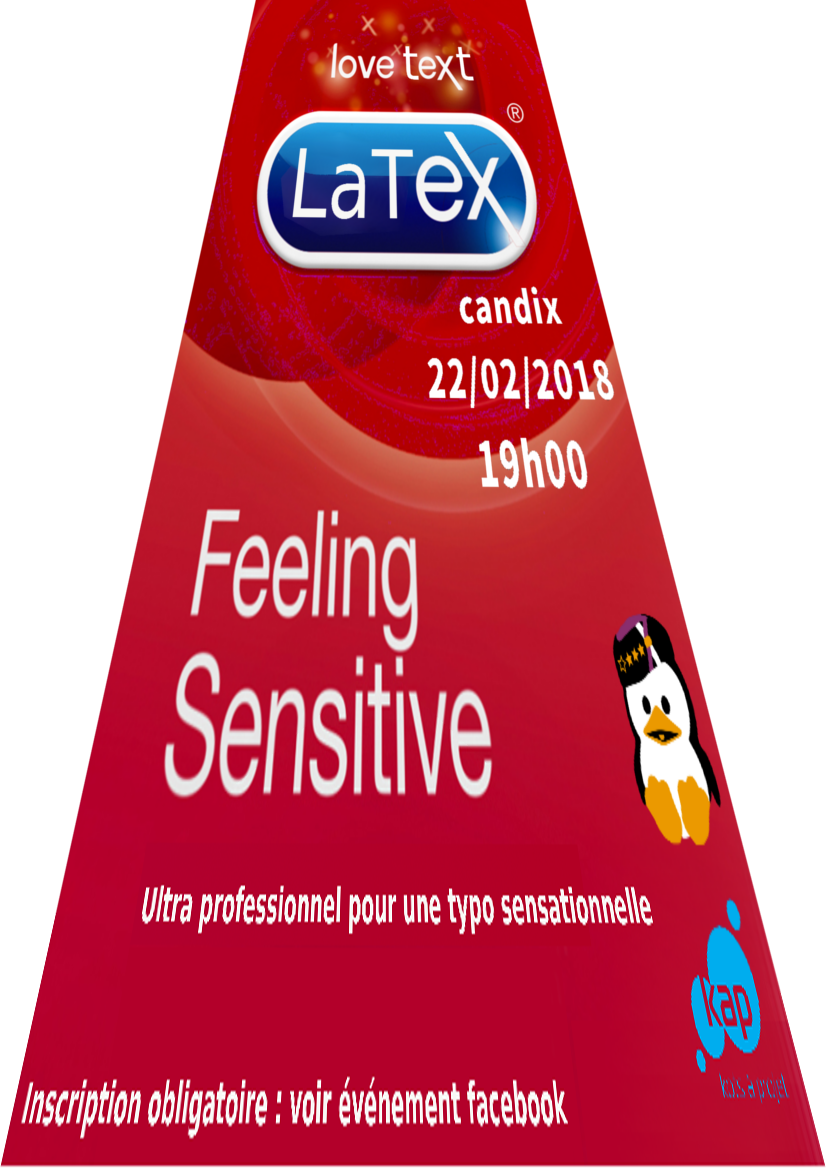
\includegraphics[width=0.5\textwidth]{Images/Perspective.png} 
	\end{figure}
	\end{minipage}
	\framebreak
	
	\item Découpe
	
	\begin{minipage}{0.45\textwidth}
	\begin{figure}
        	\centering
        	
\includegraphics[width=\textwidth]{Images/gimp-logo.png} 
	\end{figure}
	\end{minipage}\hfill
	\begin{minipage}{0.45\textwidth}
	\begin{figure}
        	\centering
        	
\includegraphics[width=0.6\textwidth]{Images/cut.png} 
	\end{figure}
	\end{minipage}
\end{enumerate}
\end{frame}

\begin{frame}{Les outils de colloration}

\textbf{Couleurs actives}

\begin{overprint}
\begin{figure}
	\centering
	\begin{tikzpicture}[scale=0.7, transform shape]
        \node[anchor=south west,inner sep=0] at (0.4,0) {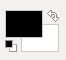
\includegraphics[width=0.1\textwidth]{Images/gimp_couleurs_actives}};
        \onslide<2>{\draw[teal,ultra thick,rounded corners] (0.25,0.3) rectangle (1.5,1); 
        \node [anchor=center, teal] (note) at (0.7,1.4) {\Large Avant-plan \textcolor{black}{{\small (Clic \textbf{gauche})}}};}
	\onslide<3>{\draw[red,ultra thick,rounded corners] (0.6,0) rectangle (1.55,0.7);
        \node [anchor=center, red] (Inner) at (0.7,-0.3) {\Large Arrière-plan \textcolor{black}{{\small (Clic \textbf{droit})}}};}
    	\end{tikzpicture} 
	%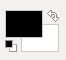
\includegraphics[width=0.1\textwidth]{Images/gimp_couleurs_actives}
\end{figure}

\vspace{-0.6cm}
\textbf{Palette des couleurs} Double clique sur l'une des couleurs actives


%\begin{figure}
%	\centering
%	\begin{tikzpicture}[scale=1, transform shape]
%        \node[anchor=south west,inner sep=0] at (0.4,0) {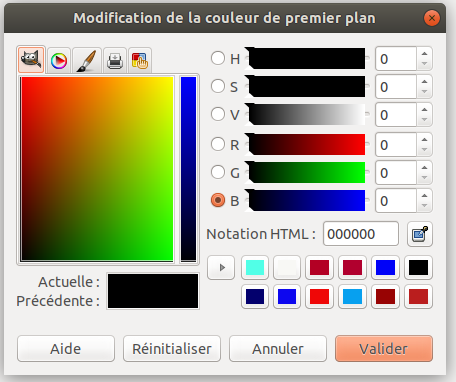
\includegraphics[width=0.4\textwidth]{Images/gimp_color_box}};
%
%        \onslide<4>{\draw[red,ultra thick,rounded corners] (4.2,1.2) rectangle (4.6,1.6); 
%        \node [anchor=center, red] (note) at (3.7,0.5) {\Large Sélection \\de couleur};}
%    \end{tikzpicture} 
%	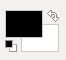
\includegraphics[width=0.1\textwidth]{Images/gimp_couleurs_actives}
%\end{figure}
\end{overprint}

\end{frame}

\begin{frame}{Les outils de colloration}
\begin{minipage}[t]{0.49\textwidth}
	\textbf{Code HTML}
	
	\vspace{0.2cm}
	Couleurs pré-définies
	
	\vspace{0.2cm}
	
	\begin{center}
	\fbox{\parbox{0.7\linewidth}{%
	\url{https://www.toutes-les-couleurs.com/code-couleur-html.php}	
	}}
	\end{center}

\end{minipage}\hfill
\begin{minipage}[t]{0.49\textwidth}
	\textbf{Code RGB}
	
	\begin{itemize}
		\item[H] Teinte
		\item[S] Valeure 
		\item[V] Saturation
		\item[R] Rouge
		\item[G] Vert 
		\item[B] Bleu
	\end{itemize}
	
\end{minipage}

\end{frame}

%\begin{frame}{L'outil de texte}

%\end{frame}

\begin{frame}{Autres outils}
\begin{enumerate}
	\item Zoom \keys{Z}
	\item Déplacement \keys{M}
	\item Alignement \keys{Q}
\end{enumerate}
\end{frame}

\begin{frame}{Les mesures}
\begin{itemize}
	\item \textbf{Echelle graduée} aux \textit{extrémités} de l'image
	
	\begin{figure}
        	\centering
        	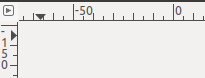
\includegraphics[width=0.3\textwidth]{Images/Scale.png} 
	\end{figure}
	
	\item Outil de mesure \keys{Maj + M}
	
	\begin{minipage}{0.45\textwidth}
	\begin{figure}
        	\centering
        	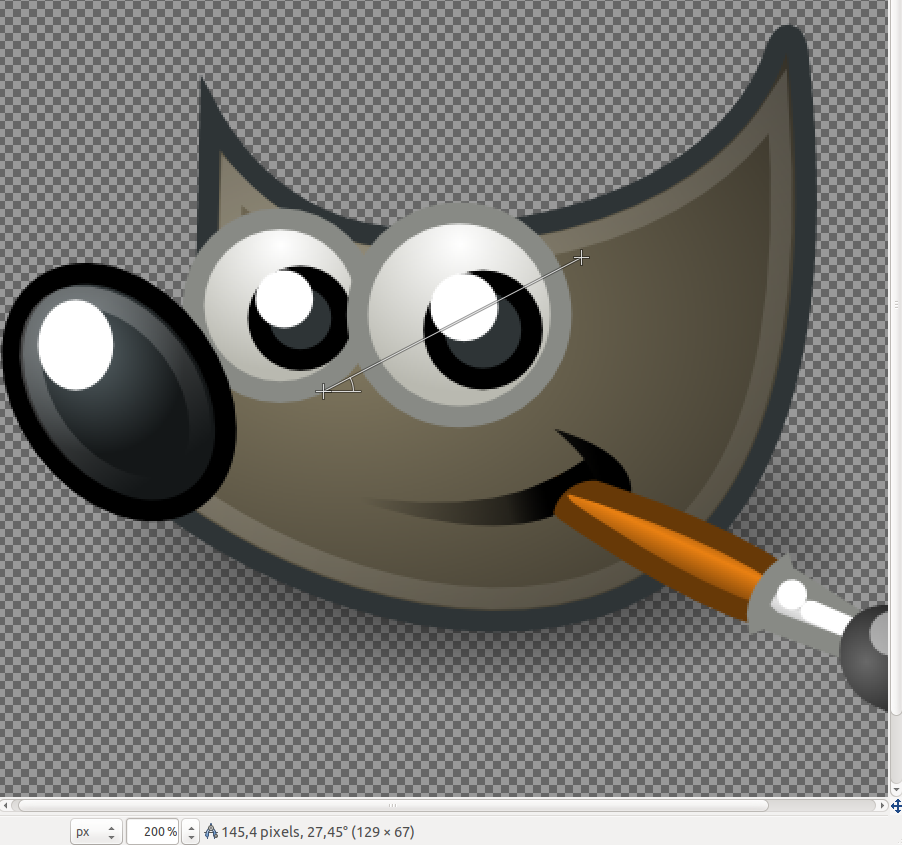
\includegraphics[width=0.8\textwidth]{Images/Measure_2.png} 
	\end{figure}
	\end{minipage}\hfill
	\begin{minipage}{0.45\textwidth}
	\begin{figure}
        	\centering
        	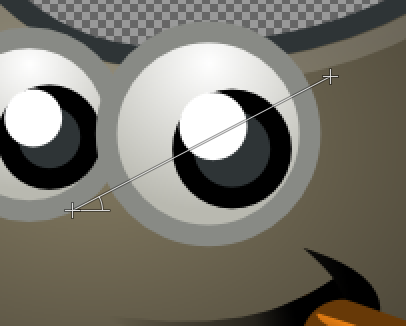
\includegraphics[width=0.6\textwidth]{Images/Measure.png} 
	\end{figure}
	\end{minipage}
\end{itemize}
\end{frame}

\begin{frame}[allowframebreaks]{Les calques}
	\begin{figure}
        	\centering
        	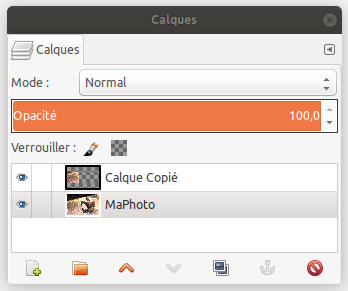
\includegraphics[width=0.3\textwidth]{Images/gimp_calques}
        	%\caption{Fenêtre de calques de GIMP} 
    	\end{figure}
    	
	\textbf{Accès} Fenêtres > Calques
	
	\vspace{0.2cm}
	\textbf{Raccourci} \keys{\ctrl + L}
	
	\framebreak
	
	\begin{figure}
        	\centering
        	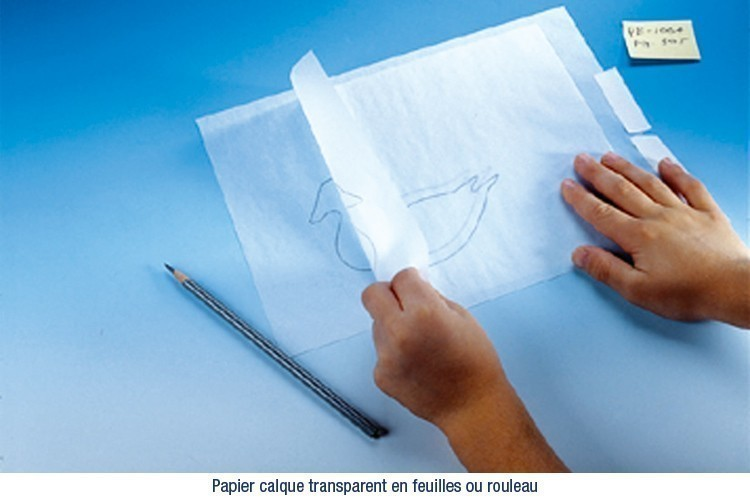
\includegraphics[width=0.5\textwidth]{Images/Calque.jpg}
    	\end{figure}
	
	\begin{itemize}
		\item \textbf{Superposition} d'images
		\begin{itemize}
			\item \textit{Avant-plan} : le plus haut
			\item \textit{Arrière-plan} : le plus bas
		\end{itemize}
		\item Visible ou non 
		\item Ancrable
		\item Indépendant
	\end{itemize}	
	
	%\begin{enumerate}
	%	\item Chaque calque s'utilises \textbf{Indépendemment}
	%\end{enumerate}

\end{frame}

\begin{frame}
	\todo[inline]{Exercices : .text, contourner automatiquement, texte "3D"}
\end{frame}

%%% MASQUES de FUSION%%
\section{Masques de Fusion}
	\begin{frame}{Masques de Fusion}
		Les masques de fusion permettent de cacher une certaine partie d'un calque.
		$\Rightarrow$ Clic droit sur le calque $\rightarrow$ Add Layer Mask ...
		
		Conseil: Sélectionnez d'abord la zone à masquer.
		\begin{center}
			\begin{figure}		
				\includegraphics[scale=.15]{Images/mask/mask1} 				
			\end{figure}	
		\end{center}
	\end{frame}

	\begin{frame}{Masques de Fusion}
		Il suffit maintenant de dessiner en noir ou blanc sur le masque de fusion pour faire apparaitre (ou disparaitre) certaines zones du calque!
		\begin{itemize}
			\item Blanc $\Longrightarrow $ opaque
			\item Noir $ \Longrightarrow $ transparent
		\end{itemize}
		\begin{center}
			\begin{figure}
				\includegraphics[scale=.15]{Images/mask/mask3}		
			\end{figure}
		\end{center}
	\end{frame}
	
	\begin{frame}{Masques de Fusion}
		\framesubtitle{Quel intérêt?}
		Faire des montages! Vous pouvez maintenant rajouter un fond à votre motif prédécoupé et le bidouiller un peu pour que ça ne se voit pas! 
		\begin{center}
			\begin{figure}
				\includegraphics[scale=.1]{Images/mask/Conference_Solvay}			
				\caption{\scriptsize{1927 Solvay Conference on Quantum Mechanics. Photograph by Benjamin Couprie, Institut International de Physique Solvay, Brussels, Belgium}}
				\end{figure}
		\end{center}
	\end{frame}

%% PURGES STALINIENNES %%
\section{Enlever un élément de l'image}
	\begin{frame}{Enlever un élément de l'image}
		Dupliquer le calque pour éviter d'endommager l'original et recouvrir la zone à éliminer avec le tampon de clonage
		\begin{itemize}
			\item Touche \textbf{C}
			\item Touche \textbf{Ctrl} pour sélectionner la zone qui sera clonée
		\end{itemize}
		\begin{center}
			\begin{figure}
				\includegraphics[scale=.15]{Images/purge/purge3} 
			\end{figure}
		\end{center}				
	\end{frame}

	\begin{frame}{Enlever un élément de l'image}
		Appliquer un masque le cas échéant et adoucir les contours avec l'outil correcteur (\textbf{B}). Changer de typer de masque de fusion peut aussi s'avérer utile.
		\begin{center}
			\begin{figure}
				\includegraphics[scale=.15]{Images/purge/purge5} 
			\end{figure}
		\end{center}				
	\end{frame}
	
	
	\begin{frame}{Enlever un élément de l'image}

		\begin{figure}[H]
			\centering
			\begin{minipage}{.5\textwidth}
				\centering
				\includegraphics[width=.5\linewidth, height=100px]{Images/purge/Apollo_15_flag,_rover,_LM,_Irwin}
				\caption{Apollo 15 Lunar Module Pilot James Irwin salutes the U.S. flag.}
			\end{minipage}%
			\begin{minipage}{.5\textwidth}
				\centering
				\includegraphics[width=.5\linewidth, height=100px]{Images/purge/Apollo_15_flag,_rover,_LM}
				\caption{Apollo 15 Lunar Module Pilot James Irwin does not salute the U.S. flag.}
			\end{minipage}
		\end{figure}

	\end{frame}


%% FILTRES %%
\section{Filtres}
	\begin{frame}{Filtres}
		\begin{itemize}
			\item S'appliquent sur un calque ou un masque
			\item Gestion 
				\begin{itemize}
				\item du flou
				\item des couleurs
				\item "d'amélioration"
				\item "artistiques"
				\item etc
				\end{itemize}
			\item "Destructifs" et non modifiables par la suite $\rightarrow$ devrait changer avec GIMP 3.2
		\end{itemize}
	\end{frame}
		
	\begin{frame}{Filtres}
		\framesubtitle{Et donc, Jamy, comment on applique un filtre?}		
		Et bien c'est facile! Il suffit de: 
		\begin{enumerate}
			\item Dupliquer le calque sur lequel on va travailler
			\item Masquer le nouveau calque afin que seule la zone qu'on souhaite modifier soit touchée par le filtre
			\item Accéder aux filtres par le menu ou un clic droit
			\item Jouer avec les réglages du filtres et l'appliquer sur le calque
		\end{enumerate}

		Conseil: si on se rend compte qu'on n'a pas appliqué les bonnes options au filtre; il n'est pas nécessaire de tout recommencer au début. Il suffit d'annuler ce qu'on vient de faire (Ctrl+Z ou "Edition $\rightarrow$ Annuler") et de réafficher le dernier (Maj+Ctrl+F ou "Filtres $\rightarrow$ Réafficher le dernier").		
		
	\end{frame}

	\begin{frame}{Filtres}
		\framesubtitle{Mais, à quoi ça sert Jamy?}
		On peut par exemple appliquer un filtre de flou Gaussien à un masque, pour rendre son intégration à un montage plus discrète:
		\begin{figure}[H]
			\centering
			\begin{minipage}{.5\textwidth}
				\centering
				\includegraphics[width=.5\linewidth, height=100px]{Images/filters/astronaut1} 
				\caption{Sans filtre appliqué}
			\end{minipage}%
			\begin{minipage}{.5\textwidth}
				\centering
				\includegraphics[width=.5\linewidth, height=100px]{Images/filters/astronaut2} 
				\caption{Après application du filtre}
			\end{minipage}
		\end{figure}		
		
		
	\end{frame}

	\begin{frame}{Filtres}
		Il existe une foule d'autres filtres, certains aux effets relativement discrets ou plus "spectaculaires":
		
		\begin{figure}[H]
			\centering
			\begin{minipage}{.3\textwidth}
				\centering
				\includegraphics[width=1\linewidth]{Images/filters/motion_blur.JPG} 
				\caption{motion blur}
			\end{minipage}
			\begin{minipage}{.3\textwidth}
				\centering
				\includegraphics[width=1\linewidth]{Images/filters/pixelize.JPG} 
				\caption{pixelize}
			\end{minipage}
			\begin{minipage}{.3\textwidth}
				\centering
				\includegraphics[width=1\linewidth]{Images/filters/ripples.JPG} 
				\caption{ripples}
			\end{minipage}
		\end{figure}
			
		\begin{figure}[H]
			\centering
			\begin{minipage}{.3\textwidth}
				\centering
				\includegraphics[width=1\linewidth]{Images/filters/old.JPG} 
				\caption{old}
			\end{minipage}
				\begin{minipage}{.3\textwidth}
				\centering
				\includegraphics[width=1\linewidth]{Images/filters/predator.JPG} 
				\caption{predator}
			\end{minipage}
			\begin{minipage}{.3\textwidth}
				\centering
				\includegraphics[width=1\linewidth]{Images/filters/photocopy.JPG} 
				\caption{photocopy}
			\end{minipage}		
		\end{figure}		
	\end{frame}


%% COULEURS %%
\section{Couleurs}
%gestion des couleurs, color blending, ...
	\begin{frame}{Gestion des Couleurs}
	gestion des couleurs, color blending, ...
	\end{frame}




%% TEXTE AVANCÉ %%
\section{Texte Avancé}
	\begin{frame}{Texte Avancé}
		Texte 3D, remplir un texte avec une texture, texte ondulé, ombre sous le texte, etc
	\end{frame}









	\begin{frame}
		\todo[inline]{Exercices : .text, contourner automatiquement, texte "3D"}
	\end{frame}

\appendix 

\begin{frame}
	\textbf{Récapitulatif des raccourcis}
	\begin{itemize}
	%todo A CLASSER (ex: view, selection, tools, ...)
	\item \keys{Ctrl + B} : Boite à outils
	\item \keys{Ctrl + L} : Fenêtre de Calques
	\item Raccourcis classiques 
	\begin{itemize}
	 \item \keys{Ctrl + A} : Tout sélectionner
	 \item \keys{MAJ + Ctrl + A} : Tout déselectionner
	 \item \keys{Ctrl + C} : Copier
	 \item \keys{Ctrl + V} : Coller
	 \item \keys{Ctrl + I} : Inverser la sélection
	\end{itemize}
	\item \keys{{+}} : Zoom (+)
	\item \keys{-} : Zoom(-)
	\item \keys{1},\keys{2},\keys{3},\keys{4},\keys{5}, \keys{MAJ + 2}, \keys{MAJ + 3}, \keys{MAJ + 4}, \keys{MAJ + 5}  
	\item \keys{R} : Sélection rectangulaire 
	\item \keys{E} : Sélection élliptique 
	\item \keys{F} : Sélection libre
	\item \keys{Ctrl} (appuyé) = Sélection de couleur
	\end{itemize}
	
	\begin{center}
	\fbox{\url{http://www.gimpusers.com/gimp/hotkeys}}
	\end{center}
\end{frame}

\begin{frame}
	\textbf{Tutoriels} gimp \fbox{\url{https://docs.gimp.org/fr/}}
\end{frame}


%\begin{frame}
%	G'MIC
%\end{frame}

\begin{comment}
\begin{frame}
	Le libre rapidement 
	
	Permet de faire plein de choses cool (et rapides)
	
	Audacity,...
\end{frame}

\begin{frame}
	
	\begin{enumerate}
	\item Ouvrir une image : File/open ==> choisir l'image à ouvrir 
	
	Ou ... plus simple : faire glisser l'image sur l'environnement de travail
	
	\item Créer un nouveau projet ==> format .xcf
	
	\item Pour obtenier une image en format "commun" ==> File/Export as ==> choisir le nom de fichier et l'extension (.png, .jpeg, .pdf, .text, .gif, .ps, .psd(compatibilité photoshop),...)
	\end{enumerate}
\end{frame}

\begin{frame}
	Description rapide des fenêtres 
	\begin{enumerate}
	\item Menu
	\item Fenêtre d'outils 
	\item Fenêtre de calques 
	
	\end{enumerate}
	Environement ouvert (échelles, zone de travail)
\end{frame}

\begin{frame}
	Outils : description générale
	
	Ctrl + B pour l'ouvrir (ou windows/Toolboxes)
	
	\begin{enumerate}
	\item Double clique pour les paramètres
	\end{enumerate} 
\end{frame}

\begin{frame}
	Outils : description par outil
	
	+ Raccourcis de l'outil
	
	+ Paramètres les plus courraments utilisés
\end{frame}

\begin{frame}
	Crayon
	
	Majuscule maintenue + Clique ==> tracer une ligne droite 
\end{frame}

\begin{frame}
	Layer manager 
	
	Ctrl + L (ou windows/Layers) pour l'ouvrir
	
	$\Rightarrow$ pour masquer, superposer, mettre à l'avant plan,... 
	 
	\begin{itemize}
		\item Calque (tel quel)
		\item Texte 
		%\item Filtre (déconseillé)
	\end{itemize}
	
	Attention : modifications QUE sur les layers sélectionnés 
	
	+ Masque (= ...) 
	\todo[inline]{exemple photo (layes cachés,...)}	 
\end{frame}

\begin{frame}
	Selection editor (All, shrink, grow, invert,...)
	
	$\Rightarrow$ Clique droit/	Select/All,Invert,None,...
\end{frame}

\begin{frame}
	Canaux (alpha et différentes couleurs)
	
	Canal alpha = ??
	
	Opérations sur les couleurs (mentionner rapidement : niveaux, balances, seuils, saturation,...)
\end{frame}

\begin{frame}
	Filtres et effets (ombres sous le texte,...)
\end{frame}
\end{comment}


\end{document}
